\chapter{Resultados y discusión} \label{chap:resultados}
% Interpretar los resultados de cómo y por qué
% - ¿Por qué el modo híbrido funciona mejor que los otros?
% - La tendencia de los pesos a irse a 0 o 1
% - Limitaciones del enfoque: bot sin memoria ni planificación, etc

Este capítulo se dedica al análisis e interpretación de los resultados obtenidos durante los experimentos detallados en el capítulo \ref{chap:experimentacion}. El objetivo no es solo presentar los datos de rendimiento de forma cuantitativa, sino también ofrecer una discusión crítica sobre por qué ciertas estrategias de entrenamiento han demostrado ser más efectivas que otras. Se intentará interpretar los valores de los pesos obtenidos en los mejores individuos de los experimentos, como la tendencia a la especialización, y se discutirán las limitaciones inherentes al algoritmo del agente. Finalmente, se concluirá el capítulo resumiendo cómo estos resultados satisfacen los objetivos finales de la investigación.

\section{Análisis de las configuraciones híbridas} \label{sec:analisis_configuraciones_hibridas}
% Unlike AlphaZero, AlphaStar initially learns to imitate the moves of the best players in its database of human vs. human games; this step is necessary to solve what DeepMind's Dave Silver calls "the exploration problem": discovering new strategies would otherwise be like finding a "needle in a haystack". Agents then play each other and deploy deep reinforcement learning. These main agents also learn by playing against suboptimal "exploiter agents" whose purpose is to expose weaknesses in the main agents (Artículo BBC). \cite{leo_kelion_deepmind_2019}
% Cuando vaya a comparar resultados, hablar del problema que tuve con 100 partidas vs 5000 partidas.

En este primer experimento se evaluaron 10 configuraciones diferentes del modo híbrido, las cuales están detalladas en la tabla \ref{tab:hybrid_schedules}. Tras obtener los mejores individuos de cada configuración, se ejecutó el script de validación para obtener una medida cuantitativa del rendimiento de cada uno contra los 4 bots de referencia: PatronFavorsBot, MaxAgentsBot, MaxPrestigeBot y DecisionTreeBot. El primer resultado de este apartado vino dado por un error en la asignación de pesos del bot, el cual provocó un cambio importante en el número de partidas del script de validación. El problema era que el bot no estaba utilizando los pesos de los mejores individuos, sino los que tenía por defecto de un entrenamiento previo, pero los resultados mostraban cambios significativos en la tasa de victorias. Aproximadamente todos estaban entre el 30\% y el 40\% de victorias, lo que parecía indicar diferencias significativas en el rendimiento de los agentes. Para intentar añadir más robustez estadística a los resultados, se decidió repetir la ejecución del script varias veces, de la misma forma que se hace con los 5 entrenamientos por configuración. Al hacerlo, se notó que el orden de los mejores individuos cambiaba en cada ejecución. Con la finalidad de afinar más la evaluación, se decidió aumentar el número de partidas del script de 100 por bot a 5000 por bot, lo que generó un resultado completamente diferente. Tras aumentar el número de partidas, todos los bots tenían un 34\% de victorias, con pequeños cambios en el orden decimal. Obviamente, la razón de este resultado era que efectivamente el bot estaba usando los mismos pesos en todas las ejecuciones, y solo al aumentar el número de estas se podía apreciar que el rendimiento de los bots era el mismo. Así, el primer resultado de este capítulo enseña que las variaciones propiciadas por la aleatoriedad del entorno pueden influir significativamente en los resultados de un experimento si el tamaño de la muestra es demasiado pequeño. Tras arreglar el error en el bot, aumentar el número de partidas considerablemente y repetir por completo el experimento, sí se obtuvieron resultados consistentes durante varias ejecuciones.

La tabla \ref{tab:hybrid_results} resume los resultados de la validación tras la corrección. Está ordenada de mayor a menor según la tasa de victorias global, permitiendo identificar rápidamente las mejores configuraciones. Además del rendimiento general, se desglosa la tasa de victorias contra cada uno de los cuatro oponentes y el tiempo total de entrenamiento.

\begin{table}[H]
	\centering
	\caption{Rendimiento y tiempo de ejecución de los campeones generados por 10 configuraciones del modo híbrido, ordenados por su tasa de victorias global.}
	\label{tab:hybrid_results}
	\begin{tabular}{@{}lccccccc@{}}
		\toprule
		\textbf{ID} & \textbf{Tasa Vic. (\%)} & \textbf{Tiempo} & \textbf{Patron} & \textbf{Agents} & \textbf{Prestige} & \textbf{Tree}   \\
		\midrule
		H3          & \textbf{48.20}          & 2h 39m          & \textbf{70.0\%} & 65.3\%          & 34.3\%            & 23.3\%          \\
		H1          & 46.31                   & 2h 36m          & 69.1\%          & \textbf{68.1\%} & 27.8\%            & 20.3\%          \\
		H5          & 43.73                   & 2h 39m          & 58.4\%          & 54.1\%          & 38.2\%            & 24.1\%          \\
		H6          & 34.70                   & 2h 50m          & 42.9\%          & 20.1\%          & \textbf{53.2\%}   & 22.6\%          \\
		H4          & 34.49                   & 2h 37m          & 43.0\%          & 18.9\%          & 51.8\%            & \textbf{24.3\%} \\
		H8          & 34.16                   & 2h 39m          & 54.3\%          & 48.4\%          & 12.1\%            & 21.8\%          \\
		H7          & 33.41                   & \textbf{2h 32m} & 44.9\%          & 20.5\%          & 51.4\%            & 16.8\%          \\
		H10         & 33.25                   & 2h 40m          & 43.6\%          & 20.9\%          & 52.3\%            & 16.1\%          \\
		H2          & 32.62                   & 2h 33m          & 42.7\%          & 20.3\%          & 52.2\%            & 15.3\%          \\
		H9          & 31.85                   & 2h 34m          & 32.3\%          & 63.1\%          & 12.4\%            & 19.7\%          \\
		\bottomrule
	\end{tabular}
\end{table}

\begin{figure}[H]
	\centering
	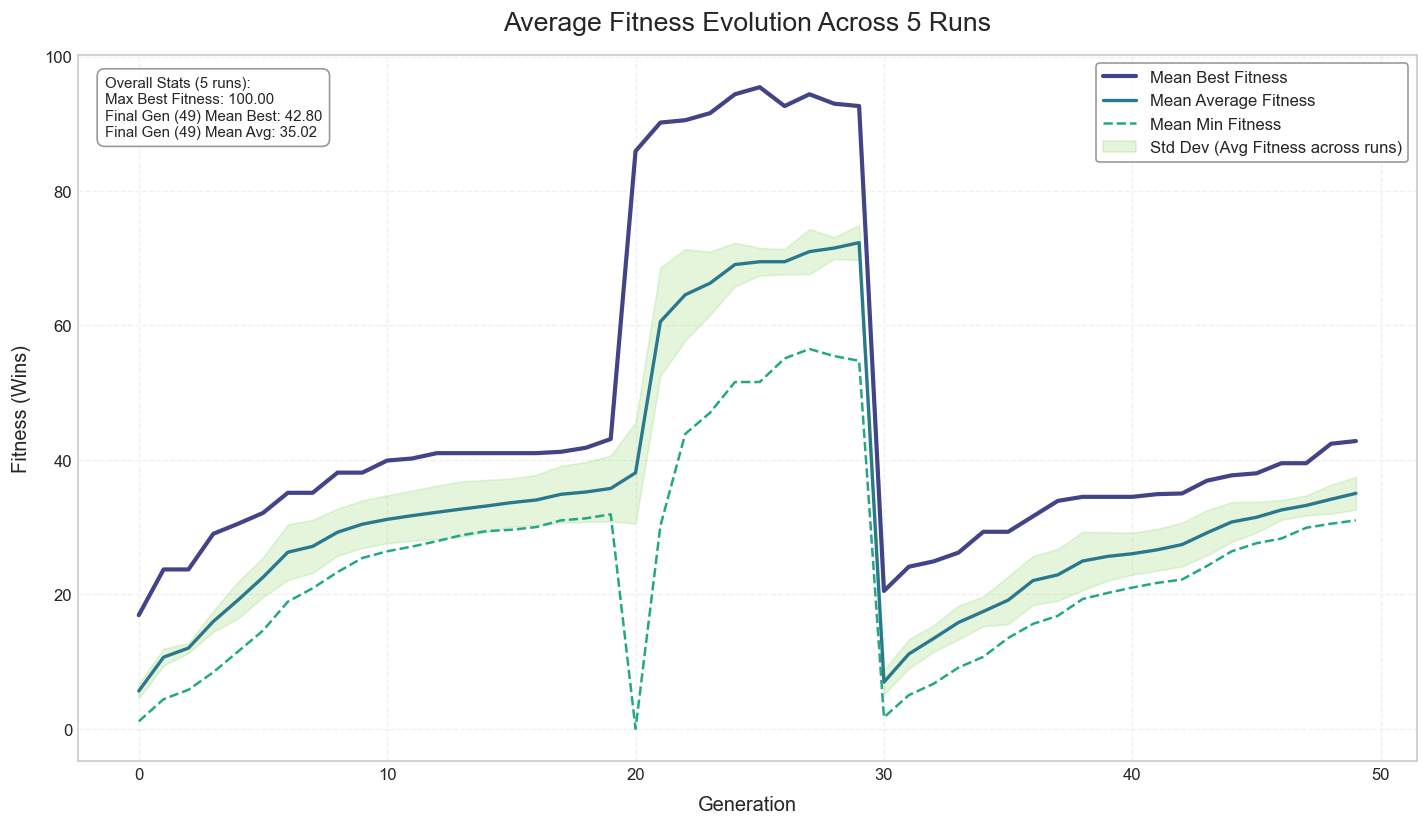
\includegraphics[width=1.0\textwidth]{img/424_fitness_evolution.png}
	\caption{Evolución del fitness sobre las generaciones para la combinación híbrida ganadora.}
	\label{fig:fitness_evolution_424}
\end{figure}

\section{Análisis de los modos de entrenamiento} \label{sec:analisis_modos_entrenamiento}

Tras la ejecución de la suite experimental que compara los modos de entrenamiento (detallada en la Tabla \ref{tab:main_experiments}), se obtuvieron 6 campeones finales, uno por cada configuración evaluada. Para determinar de forma concluyente la robustez y el rendimiento relativo de cada uno, se llevaron a cabo dos benchmarks exhaustivos: una validación contra un conjunto de bots de referencia estáticos y un torneo \textit{round-robin} de todos contra todos.

La primera fase de validación consistió en enfrentar a cada uno de los 6 campeones contra un panel de 4 bots de referencia, jugando un total de 5,000 partidas contra cada uno para asegurar la robustez estadística de los resultados. La Tabla \ref{tab:resultados_exp_modos} resume el rendimiento de cada campeón, ordenados de mayor a menor según su tasa de victorias global. Adicionalmente, se incluye el tiempo total que tomó la ejecución del experimento que produjo a cada campeón.

\begin{table}[H]
	\centering
	\caption{Rendimiento de los campeones de cada modo de entrenamiento contra oponentes fijos.}
	\label{tab:resultados_exp_modos}
	\begin{tabular}{@{}lcccccc@{}}
		\toprule
		\textbf{ID} & \textbf{Tasa Vic. (\%)} & \textbf{Tiempo} & \textbf{Patron} & \textbf{Agents} & \textbf{Prestige} & \textbf{Tree}   \\
		\midrule
		B1          & \textbf{50.89}          & 2h 53m          & 68.6\%          & \textbf{76.8\%} & 34.1\%            & 24.1\%          \\
		B5          & 48.36                   & 2h 39m          & \textbf{69.8\%} & 65.4\%          & 34.6\%            & 23.7\%          \\
		B4          & 48.27                   & \textbf{2h 27m} & 62.0\%          & 63.2\%          & 44.7\%            & 23.3\%          \\
		B2          & 41.68                   & 2h 48m          & 62.9\%          & 57.9\%          & 22.6\%            & 23.2\%          \\
		B6          & 35.01                   & 2h 34m          & 44.0\%          & 21.1\%          & 50.1\%            & \textbf{24.8\%} \\
		B3          & 32.48                   & 3h 11m          & 43.7\%          & 17.2\%          & \textbf{52.0\%}   & 17.0\%          \\
		\bottomrule
	\end{tabular}
\end{table}

Para complementar la evaluación anterior, se realizó un segundo benchmark en formato de torneo coevolutivo. En esta fase, los 6 campeones se enfrentaron entre sí en una liguilla de todos contra todos, jugando 5,000 partidas en cada emparejamiento. Este tipo de validación es fundamental para medir la capacidad de un agente para adaptarse y superar a otros oponentes que también han evolucionado, en lugar de depender únicamente de explotar las debilidades de bots con estrategias fijas.

La Tabla \ref{tab:coevo_benchmark_resultados} presenta la matriz de resultados de este torneo, mostrando la tasa de victorias de cada campeón (en filas) contra cada oponente (en columnas). Adicionalmente, la Tabla \ref{tab:coevo_ranking_final} ofrece un resumen final, ordenando a los campeones según su rendimiento global en este entorno competitivo.

\begin{table}[H]
	\centering
	\caption{Matriz de resultados del torneo EvolutionaryBot vs EvolutionaryBot.}
	\label{tab:coevo_benchmark_resultados}
	\begin{tabular}{@{}lcccccc@{}}
		\toprule
		\textbf{vs} & \textbf{B1} & \textbf{B2} & \textbf{B3} & \textbf{B4} & \textbf{B5} & \textbf{B6} \\
		\midrule
		\textbf{B1} & ---         & 41.5\%      & 22.0\%      & 40.4\%      & 47.5\%      & 23.4\%      \\
		\textbf{B2} & 58.5\%      & ---         & 3.4\%       & 44.6\%      & 51.3\%      & 4.3\%       \\
		\textbf{B3} & 78.0\%      & 96.6\%      & ---         & 99.3\%      & 77.2\%      & 61.1\%      \\
		\textbf{B4} & 59.6\%      & 55.4\%      & 0.7\%       & ---         & 50.8\%      & 3.4\%       \\
		\textbf{B5} & 52.5\%      & 48.7\%      & 22.8\%      & 49.2\%      & ---         & 26.6\%      \\
		\textbf{B6} & 76.6\%      & 95.7\%      & 38.9\%      & 96.6\%      & 73.4\%      & ---         \\
		\bottomrule
	\end{tabular}
\end{table}

\begin{table}[H]
	\centering
	\caption{Clasificación final del torneo EvolutionaryBot vs EvolutionaryBot.}
	\label{tab:coevo_ranking_final}
	\begin{tabular}{@{}lcc@{}}
		\toprule
		\textbf{ID} & \textbf{Tasa Vic. (\%)} & \textbf{Vic. Totales} \\
		\midrule
		B3          & 82.43\%                 & (20607 / 25000)       \\
		B6          & 76.25\%                 & (19063 / 25000)       \\
		B5          & 39.97\%                 & (9992 / 25000)        \\
		B1          & 34.95\%                 & (8738 / 25000)        \\
		B4          & 33.98\%                 & (8494 / 25000)        \\
		B2          & 32.42\%                 & (8106 / 25000)        \\
		\bottomrule
	\end{tabular}
\end{table}

\section{Análisis del salón de la fama} \label{sec:analisis_salon_fama}




% Decir que se han cumplido los dos objetivos faltantes:
% OG5: Evaluar cuantitativamente el rendimiento del agente entrenado mediante las diferentes estrategias, utilizando métricas relevantes.
% OG6: Analizar comparativamente la efectividad y eficiencia de las estrategias de optimización implementadas, discutiendo sus ventajas y desventajas en el contexto específico de ``Scripts of Tribute''.
% Decir que así concluye el cumplimiento de todos los objetivos específicos del proyecto.



